%!TEX program = xelatex
% Compile with XeLaTeX

\documentclass[10pt,professionalfonts,xcolor=table]{beamer}


%%%%%%%%%%
% Load style file, defaults  %
%%%%%%%%%%

\input{dom_style.tex}

%%%%%%%%%%%
% Cover slide info    %
%%%%%%%%%%%
%\setbeamertemplate{sections/subsections in toc}[sections numbered]

\title[\numu Disappearance CNN]{Muon Neutrino Disappearance in NOvA with a Deep Convolutional Neural Network Classifier}
\author[D. Rocco]{Dominick Rocco}
\date{\today}
\institute{University of Minnesota}

\begin{document}

\tikzstyle{block} = [rectangle, draw, fill=cyan!40,
   text width=3.25cm, text centered, rounded corners, minimum height=4em, minimum width = 3cm]
\tikzstyle{line}=[draw, ->, thick]
\tikzstyle{lin}=[draw, -, thick]
\tikzstyle{dot} = [minimum size=0.00pt,inner sep=0pt]
\tikzstyle{cloud} = [draw, ellipse,fill=red!50, node distance=3cm,
   minimum height=2em]

\frame{\titlepage}


\frame
{
  \frametitle{Standard Model of Particle Physics}

\begin{columns}[c]
\column{0.6\textwidth}
  \begin{itemize}
  \bang The standard model enumerates all of the fundamental particles we ``know" of
  \bang Fundamental: not comprised of other particles

  \bang \textbf{Quarks}:
    \begin{itemize}
    \bing Make up protons and neutrons...
    \bong ... and pions ($\pi$) and kaons ($K$)
    \bong ... and much much more woah

    \end{itemize}
  \bang \textbf{Leptons}:
    \begin{itemize}
    \bing Include electron ($e$) and heavier cousins muon ($\mu$) and ($\tau$)
    \bing Also includes a neutrino to compliment each one
    \end{itemize}
  \bang \textbf{Bosons}:
    \begin{itemize}
    \bing Force carriers -- mediate interactions between other particles
    \end{itemize}

  \end{itemize}
\column{0.5\textwidth}
    \begin{figure}
  \includegraphics[width=\textwidth]{figures/figures/stdmod.jpg}
  \end{figure}
\end{columns}

}


\begin{frame}
  \frametitle{Neutrino Interactions}

  \bangon
  \bang Neutrinos are very small
    \bangon
    \bing ... i.e. they rarely interact with ordinary matter
    \bing Neutral to both electromagnetic and strong forces
    \bing Billions of them are passing through you right now without interacting
    \bing Could travel through a light-year of lead and probably not interact
    \bangoff
    \bangoff
    \gap
    \begin{columns}
      \column{0.5\textwidth}
  \centering
  \textcolor{custom_red}{Charged Current}


  \includegraphics[height=0.37\textheight, angle=-90]{figures/feynman/ccNumu.pdf}
  \column{0.5\textwidth}
  \centering
   \textcolor{custom_red}{Neutral Current}


  \includegraphics[height=0.37\textheight, angle=-90]{figures/feynman/ncHad.pdf}
  \end{columns}
\gap
    \bangon
    \item Weak interactions involve either $W$ or $Z$ bozon
      \bangon
      \item $W$: charged current
      \bong ~~~~ $\nu_e \rightarrow e$ ~~ or ~~ $\nu_\mu \rightarrow \mu$ ~~ or ~~ $\nu_\tau \rightarrow \tau$
      \item $Z$: neutral current
      \bong ~~~~ $\nu_e \rightarrow \nu_e$ ~~ or ~~ $\nu_\mu \rightarrow \nu_\mu$ ~~ or ~~ $\nu_\tau \rightarrow \nu_\tau$
      \bangoff
    \bangoff

\end{frame}

\frame
{
  \frametitle{Neutrino Oscillation}
  \bangon
  \bang Neutrinos change form as they travel
	  \bangon
	  \bing ... a.k.a. neutrino oscillation
	  \bing What starts as a $\nu_\mu$ could later be observed as an $\nu_e$ or $\nu_\tau$
	  \bing Probabilities of each changes based on distance travelled and neutrino energy
	  \bangoff
  \bangoff
\begin{center}
  \begin{equation*}
  P_{\color{blue}\nu_\mu \rightarrow \nu_\mu} = 1 - \sin^2(2\theta) \sin^2\bigg(\frac{\Delta m^2 L}{4 E}\bigg)
  \end{equation*}
\gap

  \begin{columns}[c]
    \column{0.23\textwidth}
    ~
  \column{0.55\textwidth}
  \includegraphics[width=1\textwidth]{figures/figures/osc_prob.png}
  \column{0.05\textwidth}
  \vspace{-70pt}

  \begin{equation*}
  \color{blue}
  \nu_\mu
  \end{equation*}
  \vspace{-20pt}
  \begin{equation*}
  \color{red}
  \nu_\tau
  \end{equation*}
  \vspace{-17pt}
  \begin{equation*}
  \nu_e
  \end{equation*}
  \gap
  \column{0.17\textwidth}
  ~

  \end{columns}


\end{center}


}


\frame
{
  \frametitle{Neutrino Oscillation in Vacuum}
  \begin{itemize}
  \bang Neutrinos are neutral leptons that interact weakly, they are produced in one of the flavor states
  \gap
  \bang Each flavor state, $l=e,\mu,\tau$,  is a superposition of three mass states, $\nu_1$, $\nu_2$, $\nu_3$
  \gap
  \begin{equation*}
|\nu_l \rangle = \sum_{\alpha = 1,}^3 U_{l\alpha}|\nu_\alpha \rangle
  \end{equation*}
  \gap
  \bang $U_{l\alpha}$ is an element in the Pontecorvo-Maki-Nakagawa-Sakata (PMNS) matrix
  \end{itemize}

}


\frame
{
  \frametitle{PMNS Matrix}
  \begin{itemize}
  \bang $U_{l\alpha}$ is an element in the Pontecorvo-Maki-Nakagawa-Sakata (PMNS) matrix
  \begin{equation*}
 U = \begin{pmatrix} \label{pmns}
c_{13}c_{12}              &    c_{13}s_{12} 	   	 & 		s_{13} e^{-i\delta} \\
-s_{12}c_{23} - c_{12}s_{23}s_{13}e^{i\delta}	& c_{12}c_{23} - s_{12}s_{23}s_{13}e^{i\delta} 				& 		c_{13}s_{23}  \\
s_{23}s_{12} - c_{12}c_{23}s_{13}e^{i\delta}	& -c_{12}s_{23} - s_{12}c_{23}s_{13}e^{i\delta} 				& 		c_{13}c_{23}  \\
\end{pmatrix}
\end{equation*}
\gap
\bang $U$ is a unitary matrix representing a rotation in a complex 3 dimensional space
\gap
\bang $U$ depends on three Euler angles, $\theta_{12}$, $\theta_{23}$, $\theta_{13}$ and a phase $\delta$ representing CP violation
  \end{itemize}
}

\frame
{
  \frametitle{Neutrino Oscillation in Vacuum}
  \begin{itemize}
	\bang Oscillation is a result of time evolution:
	\begin{equation*}
		|\nu_l(t) \rangle = \sum_{\alpha = 1,}^3 U_{l\alpha}e^{-iE_\alpha t}|\nu_\alpha \rangle
	\end{equation*}
	\bang For relativistic neutrinos, we approximate the energy and take $t \rightarrow L$, which we substitute into the time evolution:
	\begin{equation*}
		|\nu_l(L) \rangle = e^{-iEL} \sum_{\alpha = 1,}^3 U_{l\alpha}e^{-i\frac{m_\alpha^2}{2E} L}|\nu_\alpha \rangle
	\end{equation*}
  \gap
	\bang The factor $e^{-i\frac{m_\alpha^2}{2E} L}$ gives rise to oscillation


  \end{itemize}
}

\frame
{
  \frametitle{Neutrino Oscillation in Vacuum}
  \begin{itemize}
  \bang From the last slide
	\begin{equation*}
		|\nu_l(L) \rangle = e^{-iEL} \sum_{\alpha = 1,}^3 U_{l\alpha}e^{-i\frac{m_\alpha^2}{2E} L}|\nu_\alpha \rangle
	\end{equation*}
\bang Oscillation probability is the inner product
  \begin{equation*}
P_{l\rightarrow m} = 	 \langle \nu_m|\nu_l \rangle
	\end{equation*}
	\bang We then find the oscillation probability:
	\begin{equation*}\begin{split}
P_{l\rightarrow m}(L) =  \delta_{lm} - 4  \sum_{\alpha > \beta}  \Re(U^*_{l\alpha}U_{m\alpha}U^*_{l\beta}U_{m\beta}) \sin^2 \bigg(\frac{\Delta m_{\alpha\beta}^2}{4E} L\bigg) \\
 + 2  \sum_{\alpha>\beta}  \Im(U^*_{l\alpha}U_{m\alpha}U^*_{l\beta}U_{m\beta}) \sin\bigg(\frac{\Delta m_{\alpha\beta}^2}{2E}L\bigg)
\end{split}\end{equation*}
	\bang Dynamic behavior is in sine terms, mixing angles enter through U


  \end{itemize}
}


\frame
{
  \frametitle{Current Oscillation Parameter Measurements}
    \begin{itemize}
   \bang Solar neutrino experiments have measured $\sin^2(2 \theta_{12}) $ and $\Delta m_{21}^2$
   \bang Long-baseline and atmospheric  neutrino experiments have measured $\sin^2(2 \theta_{23}) $ and $|\Delta m_{32}^2|$
   \bang $\sin^2(2 \theta_{13})$ has recently been measured to be nonzero
\bang The CP-violating phase $\delta$ has never been measured
\bang The ordering of the mass hierarchy is unknown, that is, the sign of $\Delta m_{32}^2$
\end{itemize}
\begin{columns}[c]
\column{0.5\textwidth} \footnotesize
\centering
\begin{tabular}{ c |  c }
Parameter & PDG Average\footnotemark \\  \hline
  $\sin^2\big(\theta_{12}\big)$&$  0.304 \pm0.014$  \\
  $\sin^2\big(\theta_{23}\big)$&$  0.514_{-0.056}^{+0.055}                  $   \\
  $\sin^2\big( \theta_{13}\big)$&$  0.0219 \pm0.0012$  \\
    $\Delta m^2_{21}       $&$ (7.53 \pm 0.18) \times 10^{-5}$ eV${}^2$ \\
  $|\Delta m^2_{32}|       $&$ (2.42 \pm 0.06 ) \times 10^{-3}$ eV${}^2$  \\
\end{tabular}
\column{0.5\textwidth}
 \begin{figure} \includegraphics[width=\textwidth]{figures/figures/hierarchy.jpg} \end{figure}
 \vspace{8pt}
\end{columns}
\footnotetext{K. A. Olive et al. Review of Particle Physics. Chin. Phys., C38:090001, 2014.}
}





\frame
{
\frametitle{\nova}

\begin{columns}[c]
\column{0.6\textwidth}

\begin{itemize}
\bang  \textbf{NuMI} is a neutrino source at Fermilab
\bong (Neutrinos at the Main Injector)
  \bangon
  \bing Mostly \numu
  \bangoff
\gap
\bang \textbf{\nova} is a neutrino oscillation experiment
\bong (NuMI Off-axis $\nu_e$ Appearance)
  \bangon
  \bing Two functionally identical detectors
  \bing 14 mrad off-axis
  \bing Narrow energy peak near 2 GeV

  \bangoff
\gap

\end{itemize}
\centering \footnotesize
\gap
\begin{tabular}{l | c | c}
& Near Detector & Far Detector  \\ \hline
Baseline (km)& 1  & 810   \\ \hline
Mass (kton) & 0.3 & 14  \\ \hline
Channels & 20,192 & 344,064  \\ %\hline
\end{tabular}

%{ \centering
%\includegraphics[width=1\textwidth]{figures/earth.png}}

\column{0.4\textwidth}
\centering
\vspace{-5pt}
\includegraphics[width=1\textwidth]{figures/figures/map.png}

\vspace{7pt}

\includegraphics[width=1\textwidth]{figures/figures/detectors.png}

\end{columns}


}

\frame
{
  \frametitle{NuMI}
    \begin{itemize}
	\bang High energy protons from are directed into a graphite target
	\bang These collisions produce a shower of particles
	\bang Shower is primarily pions and kaons
	\bang Muons are absorbed in steel plates and rock to leave behind a beam of muon-neutrinos
	\begin{figure} \includegraphics[width=0.85\textwidth]{figures/figures/numi.png} \end{figure}
\end{itemize}

}

\frame
{
\frametitle{\nova Detectors}

\bangon
\bang Basic unit of \nova detectors is an extruded PVC cell
\bang Cells are filled with liquid scintillator
\bang Wavelength-shifting fiber transmits scintillation light to readout
\bang Avalanche photo-diodes capture light output from fiber
\bangoff

\begin{columns}[c]
\column{0.15\textwidth}
 \includegraphics[width=1.4\textwidth]{figures/figures/cell.png}
\column{0.02\textwidth}
~
\column{0.83\textwidth}

\centering
 \includegraphics[width=0.85\textwidth]{figures/figures/schematic.jpg}

 {\scriptsize Illustration courtesy of Fermilab}

\end{columns}




}




\frame
{
  \frametitle{Far Detector}
  \centering
\begin{columns}[c]
\column{0.5\textwidth}
\centering
 \includegraphics[height=0.85\textheight]{figures/det_photos/det_front.jpg}

\column{0.5\textwidth}
\centering
 \includegraphics[height=0.85\textheight]{figures/det_photos/det_side.jpg}
\end{columns}
\gap
{\scriptsize Photos courtesy of Fermilab}


}

\frame
{
  \frametitle{Near Detector}
    \begin{itemize}
	\bang The Near Detector is considerably smaller
	\bang Installed in a 300 foot deep cavern at Fermilab

\end{itemize}
	\begin{figure} 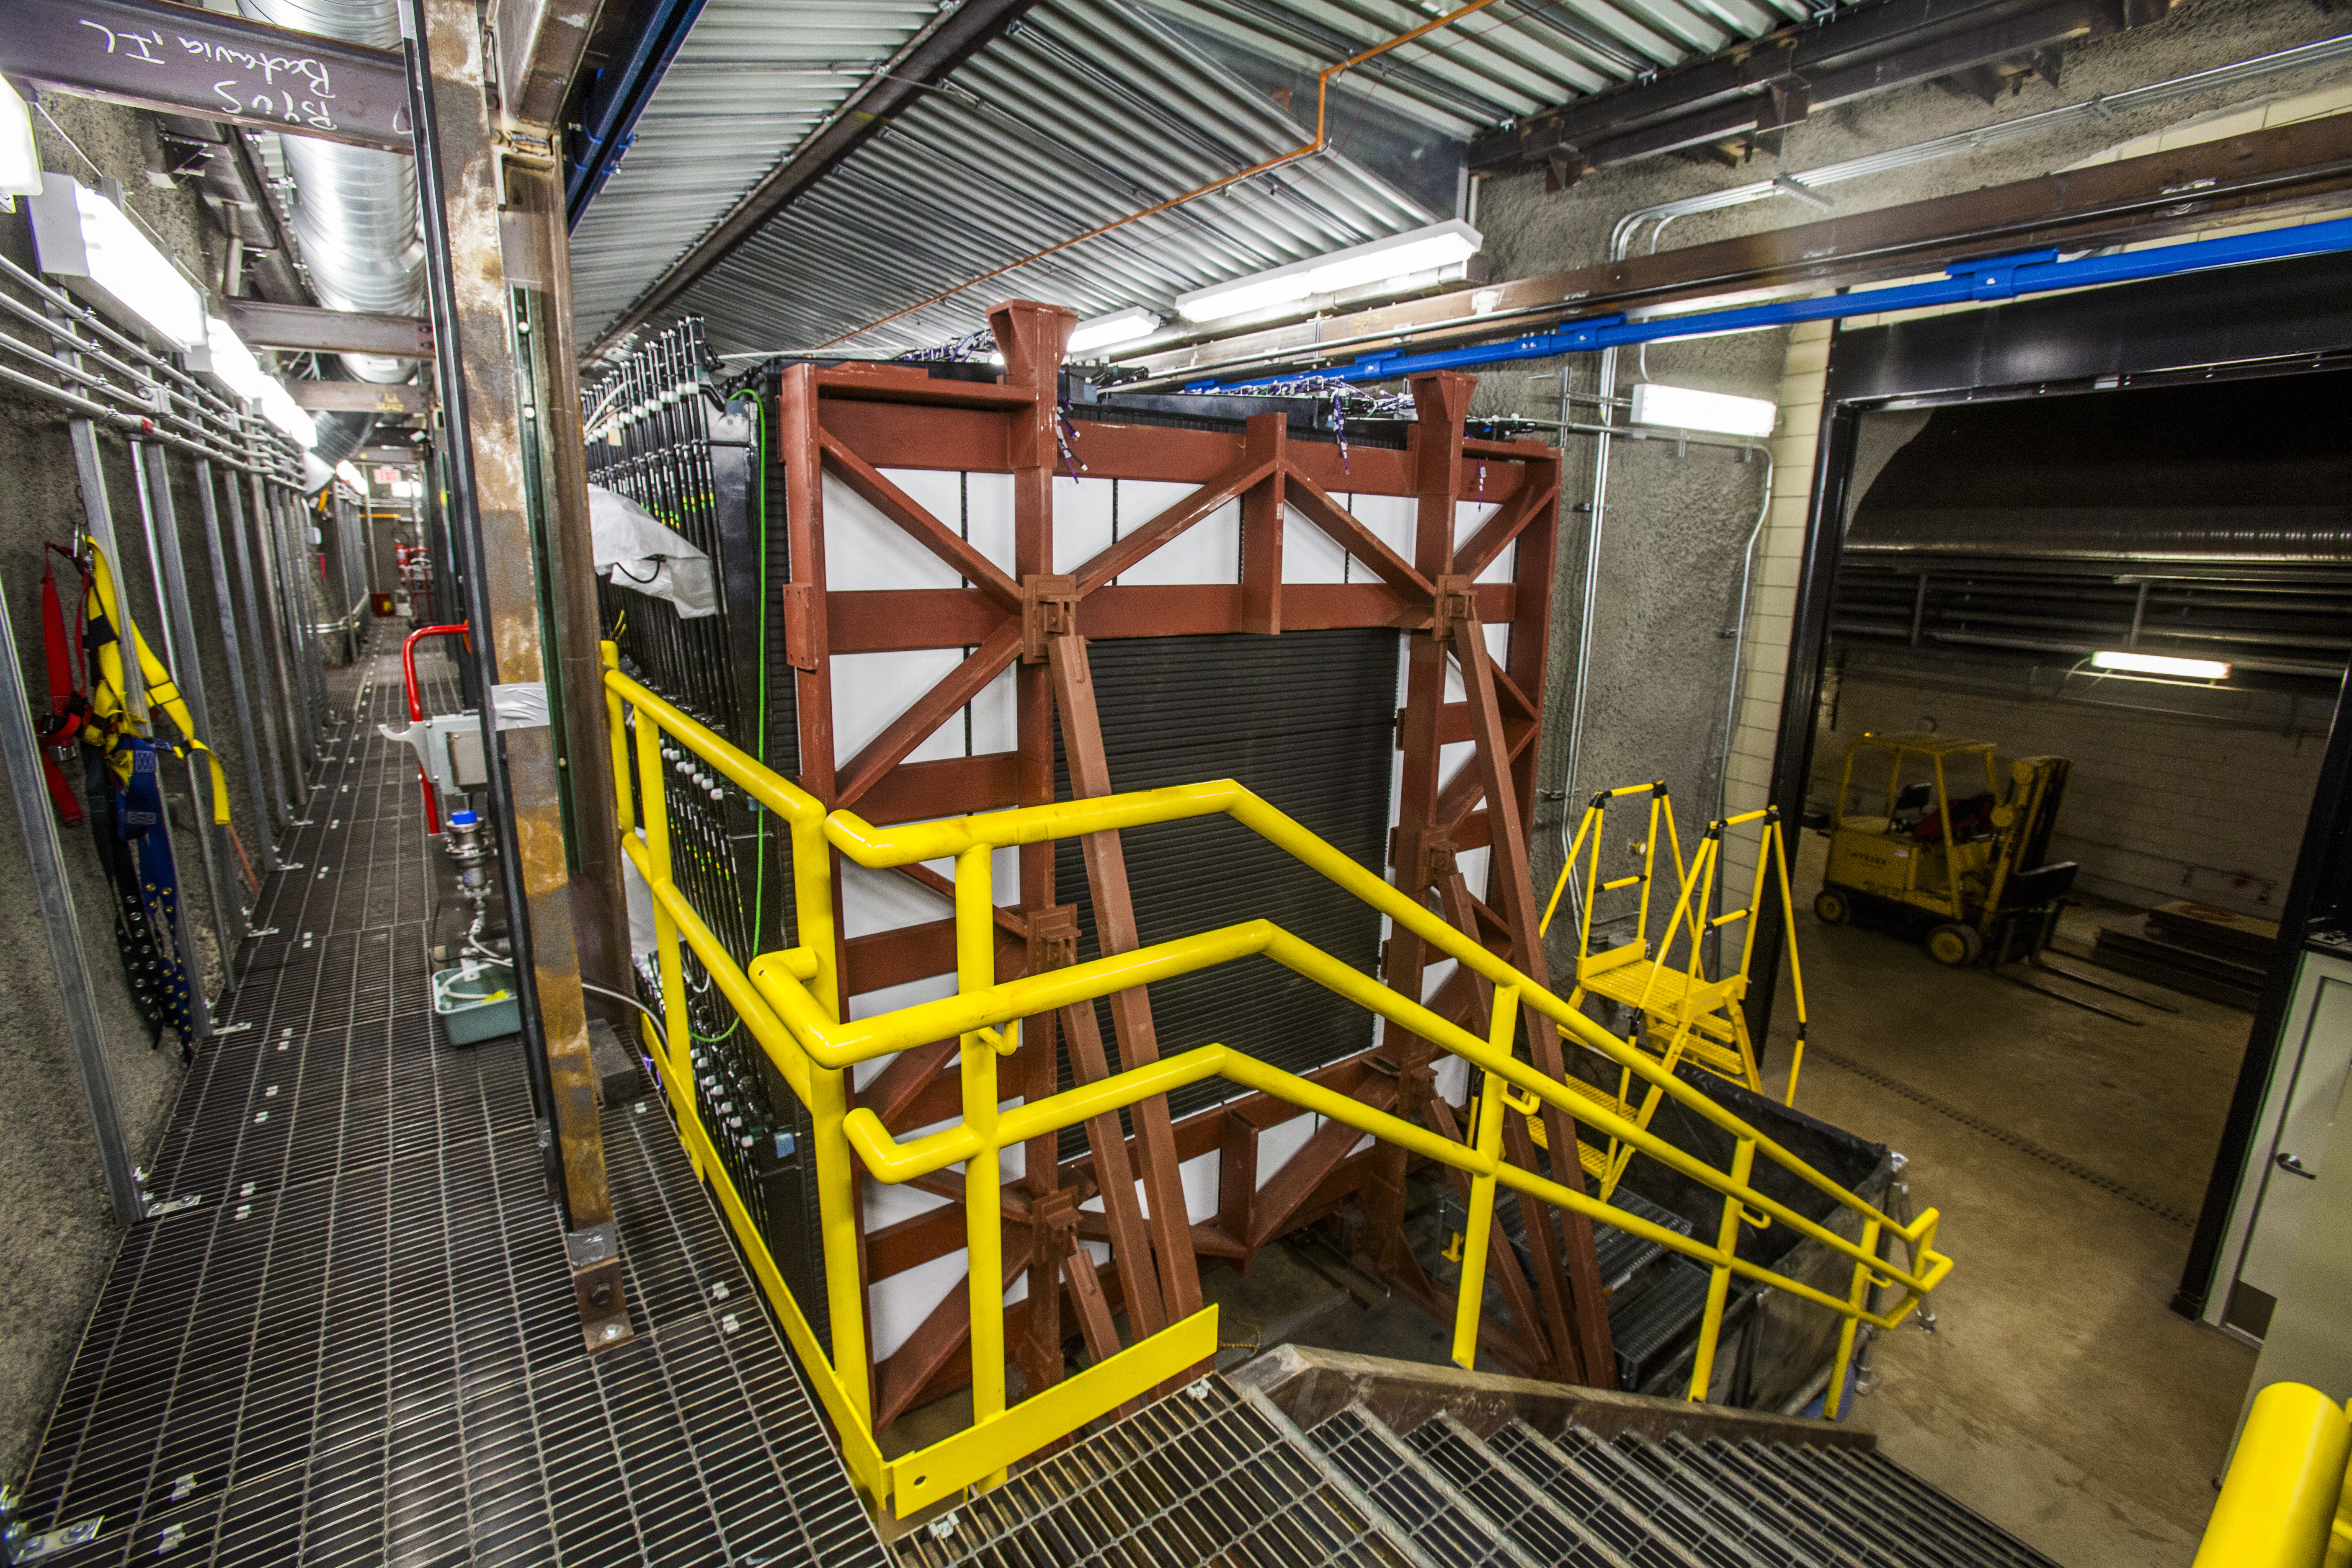
\includegraphics[height=0.55\textwidth]{figures/det_photos/ND.jpg} \end{figure}
}


\frame
{
  \frametitle{Near Detector}
	\begin{figure} \includegraphics[height=0.55\textwidth]{figures/det_photos/meND_small.jpg} \end{figure}
}

\frame
{
  \frametitle{Event Topologies}

 \begin{figure} \includegraphics[width=0.95\textwidth]{figures/figures/event_topology_nue.pdf} \end{figure}
}


\frame
{
  \frametitle{Real Far Detector Data}

 \begin{figure} \includegraphics[width=0.9\textwidth]{figures/evd_steps/evd_top_side.png} \end{figure}
}

\frame
{
  \frametitle{Real Far Detector Data}

 \begin{figure} \includegraphics[width=0.9\textwidth]{figures/evd_steps/evd_beam_dir.png} \end{figure}
}

\frame
{
  \frametitle{Real Far Detector Data}

 \begin{figure} \includegraphics[width=0.9\textwidth]{figures/evd_steps/evd_beam_dir_nu.png} \end{figure}
}

\frame
{
  \frametitle{Real Far Detector Data}

 \begin{figure} \includegraphics[height=0.9\textwidth, angle=-90]{figures/evd_steps/evd_oneslicehit.pdf} \end{figure}
}


\frame{
\frametitle{Oscillation Analysis}
\begin{tikzpicture}[]
   % Place nodes
   \node [block] (reco) {Reconstruction};
   \node [block, right = 2.7cm, right of=reco, fill=emerald] (sel) {Event Selection};
    \node [block, right = 2.7cm, right of=sel] (energy) {Energy Estimation};
    \node [block, below = 1.0cm, below of=energy] (nd) {Near Detector Data};
    \node [block, below = 2.5cm, below of=nd] (fd) {Far Detector Data};
   \node [block, left = 2.7cm, left of=nd] (eff) {Extrapolation};
   \node [block, left = 2.7cm, left of=eff] (extrap) {Prediction \\ \footnotesize{Function of oscillation parameters}};
%   \node [cloud, below =-0.5cm, below of=extrap] (fit) {Likelihood Fit};
\node[inner sep=0cm, below =2.5cm, below of=extrap, align=left] (fit)
    { \includegraphics[width=.4\textheight, angle=-90]{figures/results/fd_data_mc_numi_plots/ccE_unblind_wUnosc.pdf}};
    \node [dot, right = 1.0cm, right of=energy] (bre){};
    \node [dot, right = 1.0cm, right of=fd] (brf){};
     \node [dot, right = 1.0cm, right of=nd] (brn){};

   % Draw edges
   \path [line] (reco) |- (sel);
    \path [line] (sel) |- (energy);
    \path [lin] (energy) -- (bre);
    \path [lin] (bre) -- (brf);
    \path [line] (brf) |- (fd);
    \path [line] (brn) |- (nd);
    \path [line] (nd) -- (eff);
    \path [line] (eff) -- (extrap);
    \path [line] (extrap) -- (fit);
    \path [line] (fd) -- (fit);


\end{tikzpicture}

}


\begin{frame}

\frametitle{Reconstruction}
\framesubtitle{Slicing}

\bangon
\item First step is to resolve individual particle interactions
\gap
\item Activity is clustered in time and space to form \textit{slices}
\bangoff
\gap
\gap
\begin{columns}[b]
\column{0.5\textwidth}
\centering
\textcolor{custom_red}{Before Slicing}
\includegraphics[height=\textwidth, angle=-90]{figures/evd_steps/evd_hits.pdf}

\column{0.5\textwidth}
\centering
\textcolor{custom_red}{After Slicing}
\includegraphics[height=\textwidth, angle=-90]{figures/evd_steps/evd_slice.pdf}

\end{columns}

\end{frame}

\begin{frame}

\frametitle{Reconstruction}
\framesubtitle{Tracking}

\bangon
\item Tracking locates discrete particle trajectories
\gap
\item Two algorithms produce distinct output:
  \bangon
  \item \textit{CosmicTrack}: basic least squares regression
  \item \textit{KalmanTrack}: based on Kalman filtering
  \bangoff
\bangoff
\gap
\gap
\gap
\begin{columns}[c]
\column{0.35\textwidth}
\centering
\includegraphics[width=\textwidth]{figures/figures/tracking.jpg}

\column{0.65\textwidth}
\centering
\includegraphics[height=\textwidth, angle=-90]{figures/evd_steps/evd_track_zoom.pdf}

\end{columns}

\end{frame}


\begin{frame}

\frametitle{Reconstruction}
\framesubtitle{Prongs}
\begin{columns}[c]
\column{0.5\textwidth}
  \bangon
  \item Prongs can isolate trajectories which are less track-like
  \gap
  \item Hough transform used to find primary lines
  \gap
  \item Vertex identified based on hough lines
  \gap
  \item Prongs clustered in angular space around vertex

  \bangoff
\column{0.5\textwidth}

\centering

\includegraphics[width=\textwidth]{figures/evd_steps/slice.png}

\includegraphics[width=\textwidth]{figures/evd_steps/hough.png}

\includegraphics[width=\textwidth]{figures/evd_steps/vertex.png}

\includegraphics[width=\textwidth]{figures/evd_steps/prongs.png}

\end{columns}


\end{frame}



\begin{frame}

\frametitle{Reconstruction}
\framesubtitle{Muon ID}
\begin{columns}[c]
\column{0.55\textwidth}
  \bangon
  \item Muons tracks are identified based on KalmanTrack output
  \gap
  \item Features are extracted from tracks
    \bangon
    \item Track length
    \item Energy deposition characteristic
    \item Scattering characteristic
    \bangoff
  \gap
  \item k-Nearest Neighbors algorithm provides Muon ID score based on extracted features

  \bangoff
\column{0.45\textwidth}

\centering

\includegraphics[height=\textwidth, angle=-90]{figures/plots/reco/remid_trk_len.pdf}

\includegraphics[height=\textwidth, angle=-90]{figures/plots/reco/remid_dedxll.pdf}

\end{columns}


\end{frame}


\begin{frame}
\frametitle{Energy Estimation}
\begin{columns}[c]
\column{0.55\textwidth}
  \bangon
  \item Energy estimate is combination of muon track and hadronic energy
  \gap
  \item Muon energy estimated based on track length
  \gap
  \item Hadronic energy estimated from deposited energy of non-muon activity in slice

  \bangoff
\column{0.45\textwidth}

\centering

\includegraphics[height=\textwidth, angle=-90]{figures/plots/reco/numu_energy_muon_fit.pdf}

\includegraphics[height=\textwidth, angle=-90]{figures/plots/reco/numu_energy_had_fit.pdf}

\end{columns}


\end{frame}

\begin{frame}
\frametitle{Event Classification and Selection}

\begin{itemize}
\item Goal: analyze \numu charged-current (CC) interaction events
\gap
\item Two primary sources of background must be rejected
  \begin{itemize}
  \item Cosmic rays
  \item Other $\nu$ interactions from beam, i.e. NC and \nue CC
  \end{itemize}
\gap
\item Traditionally, classification is achieved using reconstructed features
  \begin{itemize}
  \item Criteria based on track length and other characteristics (e.g. Muon ID)
  \item Or, apply machine learning with those features
  \end{itemize}
\gap
\item But perfect reconstruction is difficult!
\gap
\item Using raw detector output could be more robust
\end{itemize}
\end{frame}

\begin{frame}
\frametitle{\nova Events as Images}

\begin{columns}[b]
\column{0.5\textwidth}

\centering
\begin{itemize}
\item \nova events are just images
  \begin{itemize}
  \item[] (two really, $X$-view and $Y$-view)
  \end{itemize}
\gap
\item Discrete pixels
\gap
\item Grayscale intensity
\end{itemize}
\vspace{20pt}
\includegraphics[width=0.85\textwidth]{figures/cnn/view_truetype6_caltype6_event155_x.pdf}


\column{0.5\textwidth}
\centering
\includegraphics[width=0.85\textwidth]{figures/cnn/view_truetype2_caltype2_event274_x.pdf}

\vspace{-5pt}


\includegraphics[width=0.85\textwidth]{figures/cnn/view_truetype13_caltype6_event144_x.pdf}

\end{columns}
\end{frame}


\begin{frame}
\frametitle{Neural Networks}
  \begin{itemize}
  \bang Artificial neural networks (ANN) do well for classification of small images
    \bangon
    \item e.g. optical character recognition (OCR)
    \item[] ... but doesn't scale well above $\sim 100$ pixels
    \bangoff
  \end{itemize}
\begin{center}
  \includegraphics[width=0.45\textwidth]{figures/figures/ocr_ann.png}
\end{center}

  \begin{itemize}
  \item Image processing community harnessing new technology
    \bangon
    \item Convolutional neural networks: good for images
    \item New training strategies: deeper networks, less overtraining
    \item GPU acceleration
    \bangoff
  \end{itemize}

\end{frame}


\begin{frame}
\frametitle{Neural Networks}

\bangon
\bang A neural network is a ``feedforward graph" of layers, $i$
  \bangon
  \item Each node,  receives input only from previous layers
  \item Nodes take input from each node in previous layer
  \item Each node passes linear combination of inputs, $z$, through a nonlinearity, $g$
  \bong \[ z_{ij} = \sum_j w_{ij} a_{(i-1)j}; ~~~~~~~~ a_{ij}  = g(z_{ij}) \]
  \bangoff
\bangoff
\vspace{20pt}
\begin{columns}[c]
\column{0.5\textwidth}

  \bangon
  \item Input layer: pixels from image
  \item Hidden layers: do the classification
  \item Output layer: classification result
  \gap
  \item Networks trained using ``backpropagation"
    \bangon
    \item Classification error is minimized in training
    \item Gradient propagated to upstream layers
    \bangoff
  \bangoff
\column{0.5\textwidth}
\centering
\includegraphics[width=1\textwidth]{figures/figures/basicNN.png}
\begin{columns}[c]
\column{0.3\textwidth}
\centering \footnotesize
Input Layer
\column{0.3\textwidth}
\centering \footnotesize
Hidden Layer
\column{0.3\textwidth}
\centering \footnotesize
Output Layer
\end{columns}
\end{columns}


\end{frame}


\begin{frame}
\frametitle{Convolutional Layers}


  \bangon
  \item Convolutional layers work well for image classification
  \bangoff
  \begin{columns}[c]
  \column{0.5\textwidth}
  \centering \includegraphics[width=0.7\textwidth]{figures/figures/conv.png}
  \column{0.5\textwidth}
  \centering \includegraphics[width=0.7\textwidth]{figures/figures/conv3d.png}
  \end{columns}
  \bangon
  \gap
  \item Convolutional filters are trained to find features in patches of the image
  \gap
  \item Filters are scanned over the input image to produce a feature map
    \bangon
    \item Upshot: position independent feature extraction
    \bangoff
  \gap
  \bangoff

\end{frame}


\begin{frame}
\frametitle{Convolutional Networks}
\begin{itemize}
  \item Many filters trained in a each convolutional layer
  \gap
  \item Pooling is a common Down-sampling technique
    \bangon
    \item ``Max pooling" simply extracts the maximum filter output (pixel intensity) from each patch
    \bangoff

  \begin{center}
 \includegraphics[width=0.5\textwidth]{figures/figures/convnet.png}
 \end{center}

\end{itemize}


\end{frame}

\begin{frame}
\frametitle{GoogLeNet and \textit{Inception}}

  \bangon
  \item GoogLeNet introduced the ``Inception module"
  \bangoff
  \begin{center}
 \includegraphics[width=0.5\textwidth]{figures/figures/inception/inception.pdf}
 \end{center}
   \bangon
  \gap
  \item Convolutional layers are arranged side-by-side rather one after another
  \item Downstream layers simultaneously learn structure at different scales
  \item $1\times1$ convolution is a tool for dimensionality reduction
    \bangon
    \item $1\times1$ convolution: constant scale factor
    \item Output filters are linear combinations of input filters
    \bangoff
  \bangoff

\end{frame}



\begin{frame}

\frametitle{\nova CNN Architecture}

  \begin{columns}
  \column{0.28\textwidth}
   \includegraphics[height=0.95\textheight]{figures/arch/arch.pdf}
  \column{0.72\textwidth}
  \begin{itemize}
  \item Separate branches for $X$ and $Y$ views
  \gap
  \item Repeated convolution, pooling, inception structures
  \gap
  \item Local Response Normalization (LRN) for smoothing
  \end{itemize}
  \end{columns}
\end{frame}




\begin{frame}
\frametitle{Event Selection}

\begin{itemize}
\item Event selection serves two purposes:
  \begin{itemize}
  \item Quality: need sufficient information to estimate energy
  \item Background rejection: need clean sample of \numu CC
  \end{itemize}
\item Containment is important for both purposes
  \begin{itemize}
  \item Events which escape detector have missing energy
  \item Cosmic rays commonly traverse entire detector (i.e. touch edges)
  \end{itemize}
\end{itemize}
\begin{center}
 \includegraphics[width=0.7\textwidth]{figures/selection/cosmicmuons.png}
\end{center}

\begin{itemize}
\item Events are required to pass a extra few criteria
\begin{itemize}
\item CNN Output
\item CosmicTrack Max-Y
\item Transverse momentum estimated from slice
\item Transverse momentum estimated from prongs

\end{itemize}
\end{itemize}
\end{frame}

\begin{frame}
\frametitle{CNN Output}

  \begin{center}
  \includegraphics[height=0.7\textwidth, angle=-90]{figures/selection/n1_cvnnumu.pdf}

  {\footnotesize(``$n-1$'' histogram -- only events which pass all other criteria)}
  \end{center}
  \bangon
  \item Select events with CNN output > 0.5
  \bangoff
\end{frame}



\begin{frame}
\frametitle{CosmicTrack start $Y$ position}

  \begin{center}
  \includegraphics[height=0.7\textwidth, angle=-90]{figures/selection/n1_cosStartY.pdf}

  {\footnotesize(``$n-1$'' histogram -- only events which pass all other criteria)}
  \end{center}
  \bangon
  \item Select events with start $Y$ < 6.0 m
  \bangoff
\end{frame}


\begin{frame}
\frametitle{Transverse momentum from slice mean}

  \begin{center}
  \includegraphics[height=0.7\textwidth, angle=-90]{figures/selection/n1_tranMom.pdf}

  {\footnotesize(``$n-1$'' histogram -- only events which pass all other criteria)}
  \end{center}
  \bangon
  \item Select events with $P_T$ < 0.8
  \bangoff
\end{frame}

\begin{frame}
\frametitle{Transverse momentum from prongs}

  \begin{center}
  \includegraphics[height=0.7\textwidth, angle=-90]{figures/selection/n1_pngptp.pdf}

  {\footnotesize(``$n-1$'' histogram -- only events which pass all other criteria)}
  \end{center}
  \bangon
  \item Select events with $P_T$ < 0.8
  \bangoff
\end{frame}

\begin{frame}
\frametitle{Selection Comparison}
  \begin{center}
   \includegraphics[height=0.7\textwidth, angle=-90]{figures/selection/cosmic_sig_osc.pdf}
  \end{center}
  \gap
  \bangon
  \item Existing \nova analysis uses muon ID and boosted decision tree (BDT)
  \gap
  \item New CNN-based selection is more efficient, especially in low energy region
  \bangoff
\end{frame}


\begin{frame}
\frametitle{Analysis}
\begin{center}
\vspace{-10pt}
\includegraphics[width=.45\textheight, angle=-90]{figures/results/spectrum_fit_systs.pdf}
\end{center}

\begin{itemize}

\item FD spectrum is fit to prediction
\gap
\item Log-likelihood for binned, Poisson distributed data
\end{itemize}
\begin{columns}[c]
\column{0.05\textwidth}
~
\column{0.4\textwidth}
\begin{equation*}
\chi^2 = 2 \sum_i e_i - o_i + o_i + \ln \big (\frac{o_i}{e_i} \big)
+ \sum_j \frac{s_{ij}^2}{\sigma_{ij}^2} 
\end{equation*}
\column{0.4\textwidth}
  \begin{itemize}
  \item[] ~
  \begin{itemize}
  \item Bins: $i$
  \item Prediction in each bin: $e_i$
  \item Observation in each bin: $o_i$
  \item Systematic uncertainties: $j$
  \item Systematic shifts: $s_{ij}$
  \item Systematic constraint: $\sigma_{ij}$
  \end{itemize}
  \end{itemize}
\end{columns}
\end{frame}


\begin{frame}
\frametitle{Extrapolation}
  \begin{center}
   \includegraphics[width=\textwidth]{figures/figures/extrap_schematic.png}
  \end{center}

  \bangon
  \item Extrapolation produces FD prediction based on ND data
  \item Accounts for for imperfect resolution in estimated energy
  \item ND/FD each have separate reco-true matrices
  \item FD/ND ratio taken from MC prediction (geometric correction)
  \bangoff
\end{frame}


\begin{frame}
\frametitle{Systematic Uncertainties}
\begin{itemize}
\item List them all
\item Talk about how analysis framework allows event records to be shifted
\end{itemize}
\end{frame}


\begin{frame}
\frametitle{Flux Uncertainty}
\begin{itemize}
\item Dem plots
\item Extrap?
\end{itemize}
\end{frame}

\begin{frame}
\frametitle{Cross Section Uncertainty}
\begin{itemize}
\item Make the combined one
\item Extrap?
\end{itemize}
\end{frame}

\begin{frame}
\frametitle{Particle Propagation Uncertainty}
\begin{itemize}
\item Slide with spectra/fits, and table
\item Another slide with combined extrap?
\end{itemize}
\end{frame}

\begin{frame}
\frametitle{Scintillation Production Uncertainty}
\begin{itemize}
\item Slide with spectra/fits, and table
\item Another slide with combined extrap?
\end{itemize}
\end{frame}

\begin{frame}
\frametitle{Calibration Uncertainty}
\begin{itemize}
\item Slide with spectra/fits, and table
\item Another slide with combined extrap?
\end{itemize}
\end{frame}


\begin{frame}
\frametitle{Detector Mass Uncertainty}
\begin{itemize}
\item Table with uncertainties
\item Muon catcher
\item Implementation
\item Another slide with combined extrap?
\end{itemize}
\end{frame}

\begin{frame}
\frametitle{Total Uncertainty}
\begin{itemize}
\item Total bands, extrapolated, prediction
\end{itemize}
\end{frame}


\begin{frame}
\frametitle{Results}
\begin{itemize}
\item Prediction without osc, with osc
\item Plot
\end{itemize}
\end{frame}

\begin{frame}
\frametitle{Event displays}
\begin{itemize}
\item Show the six from the thesis
\end{itemize}
\end{frame}

\begin{frame}
\frametitle{Result}
\begin{itemize}
\item Show spectra and contour w, w/o systs
\end{itemize}
\end{frame}

\begin{frame}
\frametitle{Feldman-Cousins}
\begin{itemize}
\item Show alternative contour
\end{itemize}
\end{frame}


\begin{frame}
\frametitle{Future}
\begin{itemize}
\item Show future contour
\item Discuss improvements
\end{itemize}
\end{frame}


\begin{frame}
\frametitle{}
\bangon
\item \nova studies neutrino oscillation with a beam and two detectors
\gap
\item Reconstruction involves machine learning and pattern recognition algorithms
\gap
\item Treating data as images with a convolutional neural network has been successful
\bangoff
\end{frame}



\frame
{
  \frametitle{Oscillation in Matter}
  \framesubtitle{Interactions}
  \begin{itemize}
  \bang In the presence of matter, neutrinos can undergo coherent scattering
  \begin{columns}[c]
  \column{0.3\textwidth}
    \centering
    \includegraphics[width=\textwidth, angle=-90]{figures/feynman/ncElec.pdf}
   \column{0.3\textwidth}
      \centering
      \includegraphics[width=\textwidth, angle=-90]{figures/feynman/ncHad.pdf}
   \column{0.3\textwidth}
      \centering
      \includegraphics[width=\textwidth, angle=-90]{figures/feynman/ccElec.pdf}

\end{columns}
\bang The neutral-current scatterings affect $\nu_e$, $\nu_\mu$ and $\nu_\tau$ equally and do not affect oscillation probabilities
\bang The charged-current interaction only occurs for $\nu_e$

\end{itemize}
}
\frame
{
  \frametitle{Oscillation in Matter}
\begin{itemize}
  \framesubtitle{Effective potential}
\bang The $\nu_e$ charged-current interaction gives rise to an effective potential:
\begin{equation*}
V_{CC} = \sqrt{2}G_F n_e
\end{equation*}
\bang The effective potential modifies the $\sin$ term in the oscillation probability:
\begin{equation*}
\sin\bigg(\frac{\Delta m_{\alpha\beta}^2}{2E}L\bigg) \rightarrow
\frac{\Delta m_{\alpha\beta}^2}{\Delta m_{\alpha\beta}^2 \pm E V_{CC}/2} \sin\bigg(\big(\frac{\Delta m_{\alpha\beta}^2}{2E} \pm \frac{EV_{CC}}{2}\big)L \bigg)
\end{equation*}
\bang The $\pm$ corresponds to neutrinos/antineutrinos
  \end{itemize}
}

\begin{frame}

\frametitle{Slicing}

\bangon
\item First step is to resolve individual particle interactions
\gap
\item Use DBSCAN for clustering, A.K.A. slicing
\gap
\item Each hit pair assigned a neighbor score with time/space distance metric
\begin{equation*}
L = \bigg( \frac{\Delta t - \Delta \vec{r} / c }{T} \bigg)^2 +
     \bigg( \frac{\Delta \vec{r}}{D} \bigg)^2
\end{equation*}
\begin{center}
 ($D$ and $T$ are configurable, $c$ is speed of light)
\end{center}
\bangoff

\begin{columns}[c]
\column{0.3\textwidth}

\centering

\includegraphics[width=\textwidth]{figures/figures/dbscan.png}

\column{0.7\textwidth}
\bangon
\gap
\item Pairs with score below threshold start a cluster
\gap
\item Cluster boundaries formed in low density regions

\bangoff

\end{columns}

\end{frame}



\begin{frame}
\frametitle{Calibration}

\bangon
\item Make a backup slide about this
\bangoff
\end{frame}


\begin{frame}
\frametitle{Regularization}

\bangon
\item Make a backup slide about this
\bangoff
\end{frame}


\begin{frame}
\frametitle{Contour Improvement}

\bangon
\item Make a backup slide about this
\item Include efficiency
\bangoff
\end{frame}


\frame
{
  \frametitle{Before Clustering}

 \begin{figure} \includegraphics[height=0.9\textwidth, angle=-90]{figures/evd_steps/evd_hits.pdf} \end{figure}
}

\frame
{
  \frametitle{After Clustering}

 \begin{figure} \includegraphics[height=0.9\textwidth, angle=-90]{figures/evd_steps/evd_slice.pdf} \end{figure}
}


\frame
{
  \frametitle{Neutrino Hypothesis and Discovery}

  \begin{columns}[c]
  \column{0.5\textwidth}
  \centering
  \includegraphics[height=0.37\textheight]{figures/figures/betaPretty.png}
  \column{0.5\textwidth}
  \centering
  \includegraphics[height=0.37\textheight]{figures/figures/betaspec.jpg}
  \end{columns}
  \gap
  \begin{itemize}
  \bang Beta decay originally ($\sim$1900) seen as two body decay: $p \rightarrow n + e^-$
  \bang Conservation of momentum predicts single-valued energy spectrum for $e^-$
  \bang The spectrum they measured was in fact continuous
  \vspace{10pt}
  \bang Wolfgang Pauli postulated an unseen third particle
  \bang Enrico Fermi dubbed it neutrino, or ``little neutral one"
  \bang Neutrinos from nuclear reactors were experimentally observed in 1956
  \end{itemize}
}


\end{document}
